%!TEX root=./LIVRO.tex
\captionsetup{font={small, it}}
\captionsetup{justification=raggedright, singlelinecheck=false}

\chapter{Apresentação}

\section{A \textit{Plataforma digital Revisa SAEB}}

% Felipe

A \textit{Plataforma digital Revisa SAEB} foi desenvolvida para alunos e
professores do 1º ao 9º ano do Ensino Fundamental. Por meio dela, os alunos
têm acesso às versões digitais do material impresso (apresentações PowerPoint), simulados 
por módulos, vídeos e jogos. Já os professores, além de terem acesso ao
mesmo conteúdo que os alunos, contam com uma série de vídeos de capacitação.
Os coordenadores por sua vez, recebem relatórios de frequência e pontuação por
e-mail ou pela plataforma.

Todo esse conteúdo da \textit{Plataforma digital} está publicado em um
sistema integrado de gestão, desenvolvido desde
2005. O sistema de código aberto, conhecido como Odoo, oferece uma ampla gama de módulos e
recursos para a educação que podem ser personalizados e adaptados às
necessidades específicas de diferentes situações. Esse mesmo sistema é usado
em todas as escolas públicas de Portugal desde 2022, para vários fins
educacionais.\footnote{ Para saber mais sobre o uso do projeto Odoo, consulte 
\href{https://www.odoo.com/pt_BR/partners/thinkopen-solutions-portugal-2614}{Thinkopen Solutions — Portugal.}}
%\url{}


Especificamente, a \textit{Plataforma} possui dois módulos que oferecem 
recursos relacionados ao \textbf{eLearning} (Cursos On-line) e 
à aplicação de questionários e provas, que fazem parte da \textit{Plataforma digital Revisa SAEB}.  




\section{Como acessar?} 

\begin{itemize}
\item URL da \textit{Plataforma Digital Revisa SAEB digital}:  \url{revisasaeb.com.br}.

\item Credenciais do aluno: \textbf{aluno-teste} e senha: \textbf{minhacidade}
\item Credenciais do professor: \textbf{professor-teste} e senha: \textbf{minhacidade}
\item Credenciais do coordenador: \textbf{coordenador-teste} e senha: \textbf
 {minhacidade}\footnote{ Caso tenha alguma dúvida ou dificuldade, favor
 entrar em contato com Elio Viniski pelo email elio@edoo.me ou
 telefone +51 9252-5268 (suporte técnico responsável). }
\end{itemize}

\section{Quais são as áreas principais da plataforma?}

Após o \textit{login}, o professor e os gestores terão acessoa duas áreas:

\begin{itemize}
\item  aos cursos de formação.
 
\item aos módulos de gestão (Cursos Online, Provas e Eventos), para relatórios. 

\item a todos os cursos dos alunos.

\item Fórum


\end{itemize}


\begin{figure}[b]
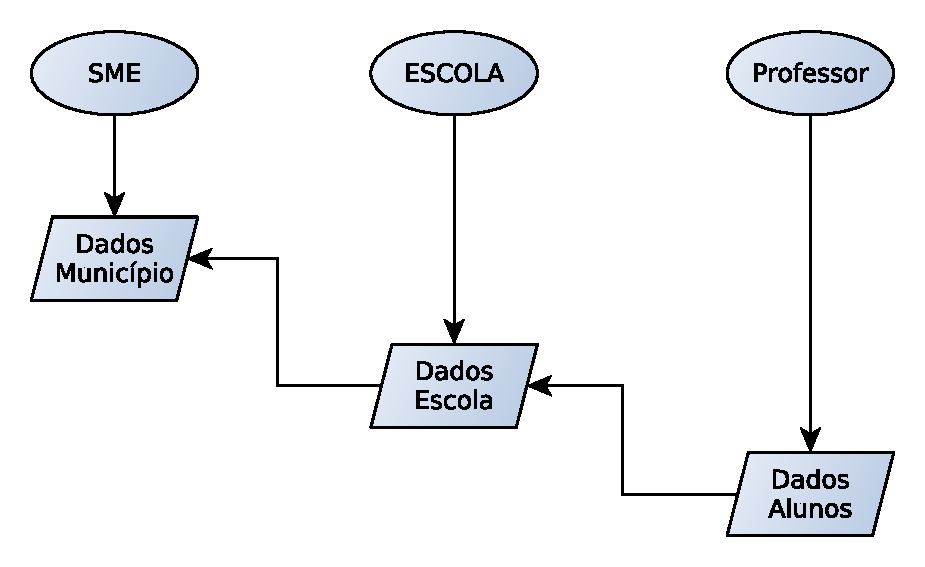
\includegraphics[width=\textwidth]{imgs/perfis_data.pdf}
\caption{Os usuários estão classificados em grupos e só têm acesso ao seu domínio}
\end{figure}


Já o aluno terá acesso a:

\begin{itemize}
\item curso do seu ano,  divididos em seções. 

\item calendário de eventos
\end{itemize}

Os relatório de frequência e desempenho fica à disposição do cooredenador e pode ser 
enviado automaticamente para o grupo de professores. 

Para testes, entre no endereço \textbf{revisasaeb.com.br} com 
as credenciais \textbf{aluno-teste} e senha \textbf{minhacidade}. 

\section{Diferenciais da \textit{Plataforma}}

\begin{figure}[h]
\includegraphics[width=\textwidth]{imgs/spec}
\caption{Home da Plataforma}
\end{figure}

E também cabe destacar ainda a \textit{gamificação} do aprendizado:
são definidos roteiros e avatares que são conquistados conforme a 
pontuação do  aluno. 

\begin{figure}[b]
\centering \includegraphics[width=0.7\textwidth]{imgs/gamification}
\caption{Visual das informações de desempenho do aluno e seu avanço e avatar.}
\end{figure}




\chapter{Imagens do site}

\mbox{}

\begin{figure}[h]
\includegraphics[width=\textwidth]{imgs/front}
\caption{Home da Plataforma}
\end{figure}

% \begin{figure}
% \includegraphics[width=\textwidth]{imgs/login}
% \caption{Tela de login}
% \end{figure}


\begin{figure}[H]
\includegraphics[width=\textwidth]{imgs/cursos}
\caption{Todos os cursos do aluno divididos por ano}
\end{figure}


\begin{figure}[H]
\includegraphics[width=\textwidth]{imgs/jogo1}
\caption{Jogo sobre frações}
\end{figure}


\begin{figure}[H]
\includegraphics[width=\textwidth]{imgs/jogo2}
\caption{Jogo sobre uso de dinheiro}
\end{figure}


\begin{figure}[H]
\includegraphics[width=\textwidth]{imgs/video1}\bigskip

\includegraphics[width=\textwidth]{imgs/video-2}
\caption{Vídeos}
\end{figure}



\begin{figure}[H]
\includegraphics[width=\textwidth]{imgs/backend_calendário-2}
\caption{Calendário de administração de eventos}
\end{figure}


\begin{figure}[H]
\includegraphics[width=\textwidth]{imgs/progresso}
\caption{No perfil do aluno é possível ver o progresso de cada curso}
\end{figure}

\begin{figure}[H]
\includegraphics[width=\textwidth]{imgs/relatorio}
\caption{Relatório detalhado por aluno}
\end{figure}


\begin{figure}[H]
\includegraphics[width=.7\textwidth]{imgs/relatorio1}
\caption{Relatório para o coordenador ou professor}
\end{figure}

% André
% Explicar as seções, a relação com o material impresso, os quiz


